% skyrius apie matematinį modelį

\section{Matematiniai modelis}

Šiame darbe yra naudojamas (YAG) reakcijos modelis, kurį pasiūlė Ivanauskas et al \cite{ivanauskasModellingSolidState2005}. Yra žinoma, kad reakcijos produktas yra kristalas ir nedifunduoja, todėl difuzijos dėmens trečioje lygtyje nėra. Šis matematinis modelis yra reakcijos-difuzijos sistema, kuriai spręsti naudojamas išreikštinių baigtinių skirtumų metodas \cite{pressNumericalRecipes3rd2007}. Procesas yra modeliuojamas dviejose dimensijose - stačiakampio srityje.

\begin{subequations} \label{rect}
	\begin{align}
		\frac{\partial c_1}{\partial t} & =-3kc_1c_2+D\left(\frac{\partial^2c_1}{\partial x^2}+\frac{\partial^2c_1}{\partial y^2}\right) \\
		\frac{\partial c_2}{\partial t} & =-5kc_1c_2+D\left(\frac{\partial^2c_2}{\partial x^2}+\frac{\partial^2c_2}{\partial y^2}\right) & (x, y, t)&\in\Omega\times[0, T]\\
		\frac{\partial c_3}{\partial t} & =2kc_1c_2
	\end{align}
\end{subequations}

Čia $c_1,c_2,c_3$ yra medžiagų koncentracija, $t$ - laikas, $T$ - proceso trukmė, $W$ - stačiakampio plotis, $H$ - stačiakampio aukštis,
$D$ - medžiagų $c_1$ ir $c_2$ difuzijos konstanta, $k$ - reakcijos greičio konstanta, $\Omega=(0, W)\times(0, H)$ - stačiakampio sritis, kurioje vyksta reakcija. Srities $\Omega$ kraštinę žymėsime $\partial\Omega$:
\begin{align*}
    \partial\Omega=\{0, W\}\times[0, H]\cup[0, W]\times\{0, H\}
\end{align*}
Šios sistemos modelis yra uždaras - medžiagos neprateka pro stačiakampio srities kraštinę $\partial\Omega$, t.~y. taikoma Neumano kraštinė sąlyga:
\begin{align} \label{general-boundary-cond}
	\nabla c_m(x, y, t)\cdot\vec{n}&=0, & (x, y)&\in\partial\Omega & t&\in[0, T] & m&=1, 2, 3
\end{align}
Čia $\nabla c_m$ yra medžiagos $c_m$ gradientas, o $\vec{n}$ - paviršiaus $\partial\Omega$ normalė. Išskleidus kraštines sąlygas \eqref{general-boundary-cond} dviejose dimensijose gauname:
\begin{equation} \label{boundary-cond}
\begin{aligned}
\begin{split}
    \frac{\partial c_m}{\partial x}\Big|_{x=0}=\frac{\partial c_m}{\partial x}\Big|_{x=W}&=0 & y&\in[0,H] & t&\in[0, T] & m&=1, 2, 3\\
    \frac{\partial c_m}{\partial y}\Big|_{y=0}=\frac{\partial c_m}{\partial y}\Big|_{y=H}&=0 & x&\in[0,W] & t&\in[0, T] & m&=1, 2, 3
\end{split}
\end{aligned}
\end{equation}

\newpage
Ruošiant medžiagas reakcijai yra sudaromas stoichiometrinis medžiagų mišinys, todėl matematiniam modeliui yra taikomos šios pradinės sąlygos:
\begin{equation} \label{intial-cond}
	\begin{aligned}
		c_1(x, y, 0) & = \begin{cases} 3c_0, & \text{jei } (x, y)\in\Omega_1 \\ 0, & \text{kitaip} \end{cases} & \Omega_1&=\big(0, \tfrac{W}{2}\big]\times\big(0, \tfrac{H}{2}\big]\cup\big[\tfrac{W}{2}, W\big)\times\big[\tfrac{H}{2}, H\big)\\
		c_2(x, y, 0) & = \begin{cases} 5c_0, & \text{jei } (x, y)\in\Omega_2 \\ 0, & \text{kitaip} \end{cases} & \Omega_2&=\big(0, \tfrac{W}{2}\big)\times\big(\tfrac{H}{2}, H\big)\cup\big(\tfrac{W}{2}, W\big)\times\big(0, \tfrac{H}{2}\big)\\
		c_3(x, y, 0)&=0 & (x, y)&\in\overline{\Omega}=\Omega\cup\partial\Omega\\.
	\end{aligned}
\end{equation}

Čia $3c_0$ ir $5c_0$ atitinkamai yra medžiagų $c_1$ ir $c_2$ dalelių tankiai.

\begin{figure}[h!]
	\centering
	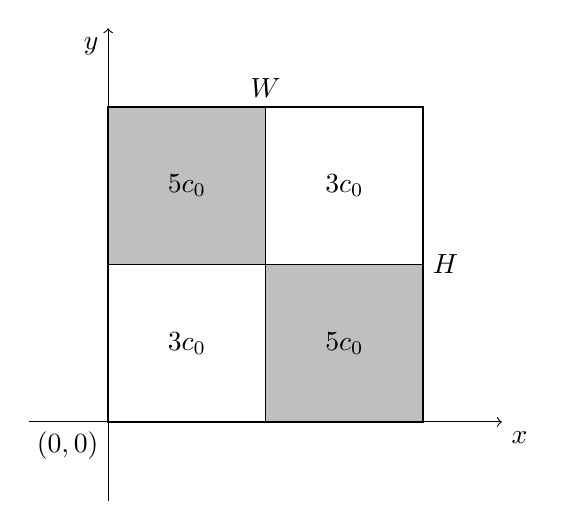
\begin{tikzpicture}[scale=2.0]
		\draw[fill=white] (0,0) rectangle (1,1);
		\draw[fill=white] (1,1) rectangle (2,2);
		\draw[fill=gray!50] (0,1) rectangle (1,2);
		\draw[fill=gray!50] (1,0) rectangle (2,1);

		% Draw the boundary of the square
		\draw[thick] (0,0) rectangle (2,2);

		% Draw axes
		\draw[->] (-0.5, 0) -- (2.5, 0) node[anchor=north west] {$x$};
		\draw[->] (0, -0.5) -- (0, 2.5) node[anchor=north east] {$y$};

		% Mark the origin
		\node[anchor=north east] at (0,0) {$(0, 0)$};

		% Mark the side length
		\draw[-] (2,0) -- (2,2) node[midway, right] {$H$};
		\draw[-] (0,2) -- (2,2) node[midway, above] {$W$};
		\draw (0.5, 1.5) node[anchor=center] {$5c_0$};
		\draw (1.5, 0.5) node[anchor=center] {$5c_0$};
		\draw (1.5, 1.5) node[anchor=center] {$3c_0$};
		\draw (0.5, 0.5) node[anchor=center] {$3c_0$};
	\end{tikzpicture}
	\caption{Sistemos pradinės sąlygos srityje $\Omega$. Tamsesnė spalva žymį sritį $\Omega_2$, o šviesesnė $\Omega_1$}
\end{figure}